\chapter{Installing Stellar Command} \label{chap:install}
Installing Stellar Command is completed in two parts: the Stellar Command module and the examples. Additionally, there the option to download the source files from Github.
\section{Downloading Stellar Command}
Download the Stellar Command archive from \url{https://github.com/angelofraietta/StellarCommand/blob/master/build/distributions/StellarCommand.zip}

Unzip the archive StellarCommand.zip into a folder. Figure~\ref{fig:zipcontents} displays the contenmts of the archive. 

\begin{figure}[htbp]
	\centering
	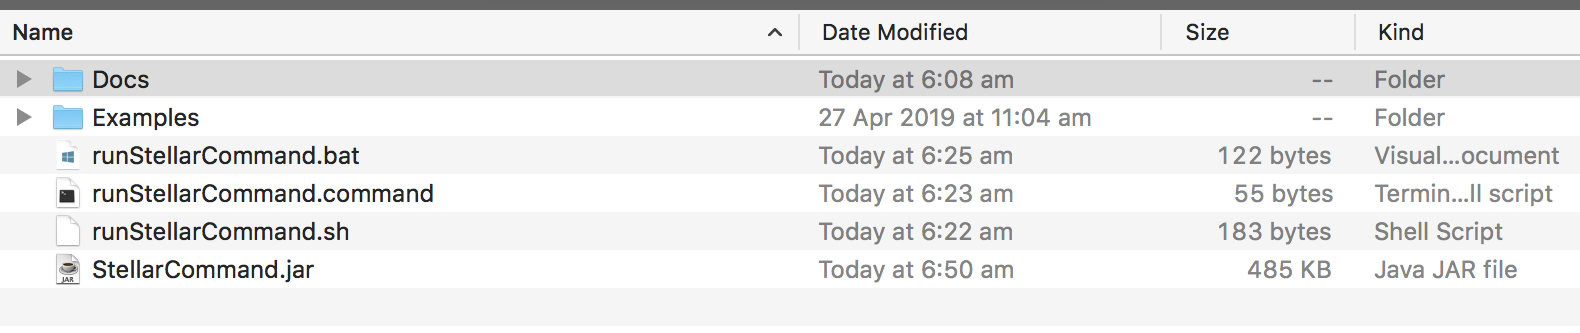
\includegraphics[width=1\columnwidth]{zipcontents}
	\caption{Stellar Command contents.}
	\label{fig:zipcontents}
\end{figure}

The \textit{Docs} folder contains the documentation files. The \textit{Examples} folder contains examples inside a \textit{HappyBrackets} project. The file \textit{StellarCommand.jar} is the Java archive that you need to include in your project if you are using it as a library. The remaining files are scripts for running in MacOS, Linux or Windows. Instructions for launching Stellar Command are in chapter~\ref{chap:launchosc} --
\emph{\titleref{chap:launchosc}}, with specifics on scripts in described in section ~\ref{sec:configscript} --
\emph{\titleref{sec:configscript}}.

\section{Setup Examples}\label{subsec:runningexamples} \index{Examples!HappyBrackets}
The examples for demonstrating Stellar Command are run using the HappyBrackets creative coding kit. In order to use the kit, you must install Java, IntelliJ and the HappyBrackets IntelliJ plugin. Instructions can be found at \url{https://github.com/orsjb/HappyBrackets/wiki/Getting-Started}.

Once you have installed HappyBrackets, open the Examples project by selecting \textit{Open Project} in IntelliJ (Figure~\ref{fig:openproject}) and then selecting the \textit{Examples} folder and pressing \textit{Open}, as shown in Figure~\ref{fig:selectproject}.

\begin{figure}[htbp]
	\centering
	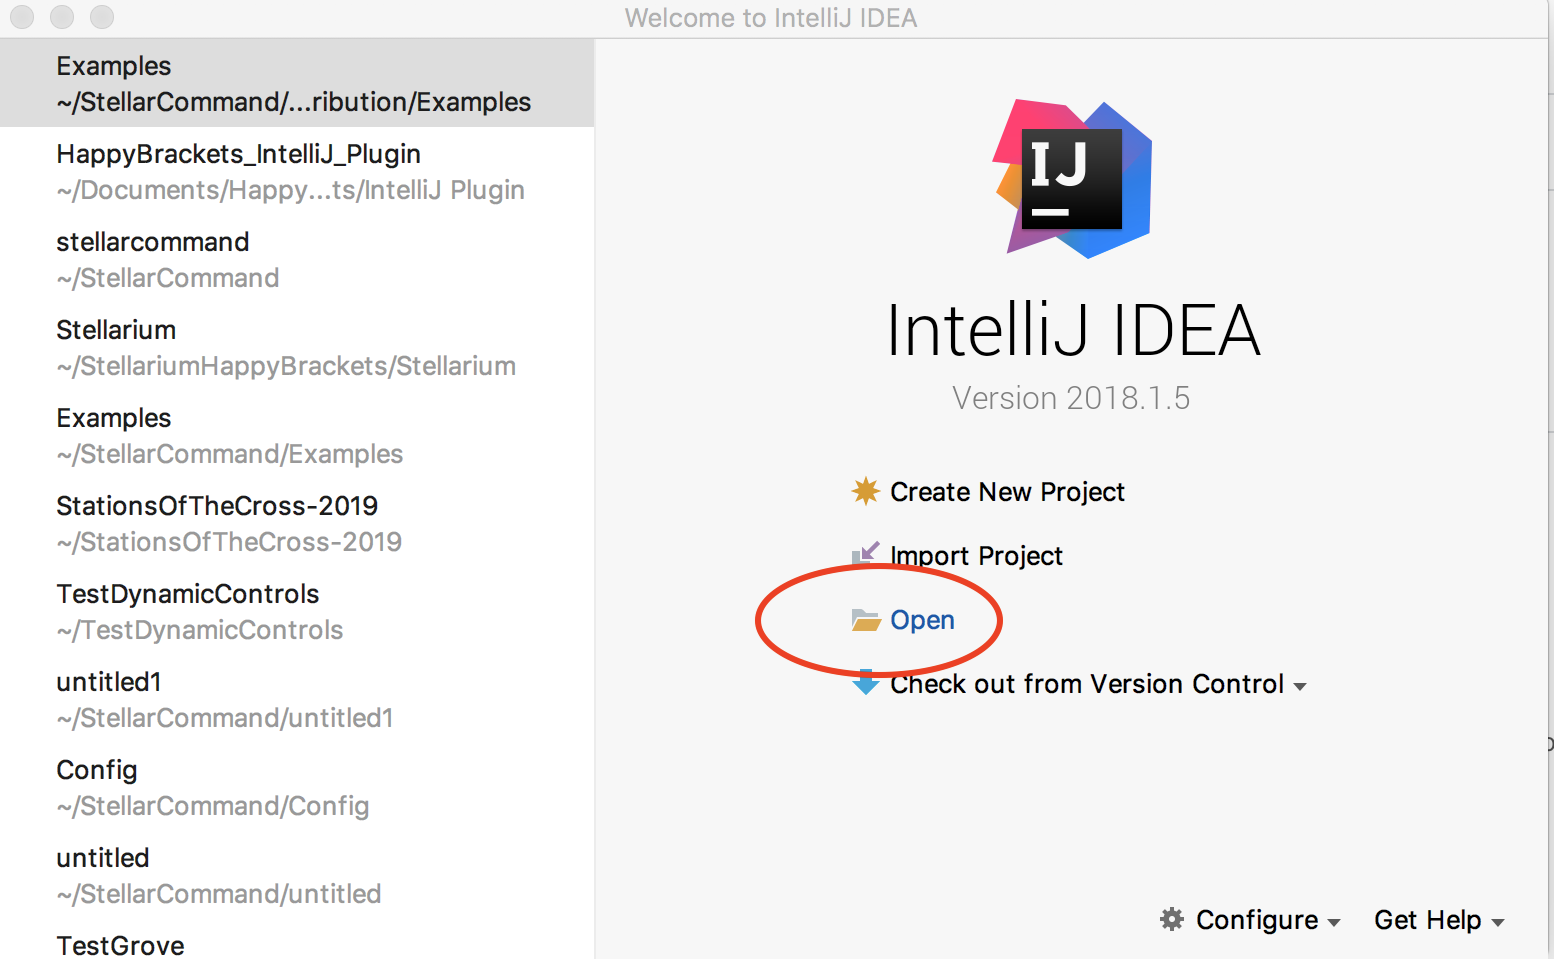
\includegraphics[width=1\columnwidth]{openproject}
	\caption{Select Open Project in IntelliJ}
	\label{fig:openproject}
\end{figure}

\begin{figure}[htbp]
	\centering
	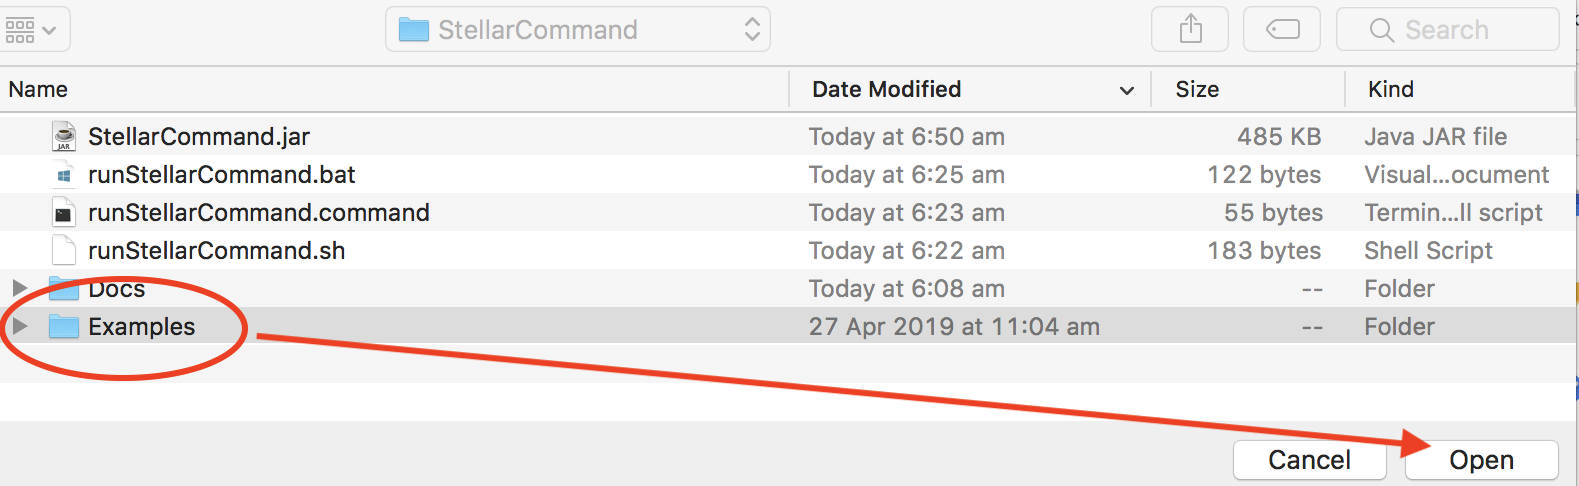
\includegraphics[width=1\columnwidth]{selectproject}
	\caption{Select Examples and press "Open"}
	\label{fig:selectproject}
\end{figure}

DO NOT enter into the \textit{Examples} folder as shown in Figure~\ref{fig:badopen} as this will not open the project. If you inadvertently get to this stage, press cancel and try again.. 

\begin{figure}[htbp]
	\centering
	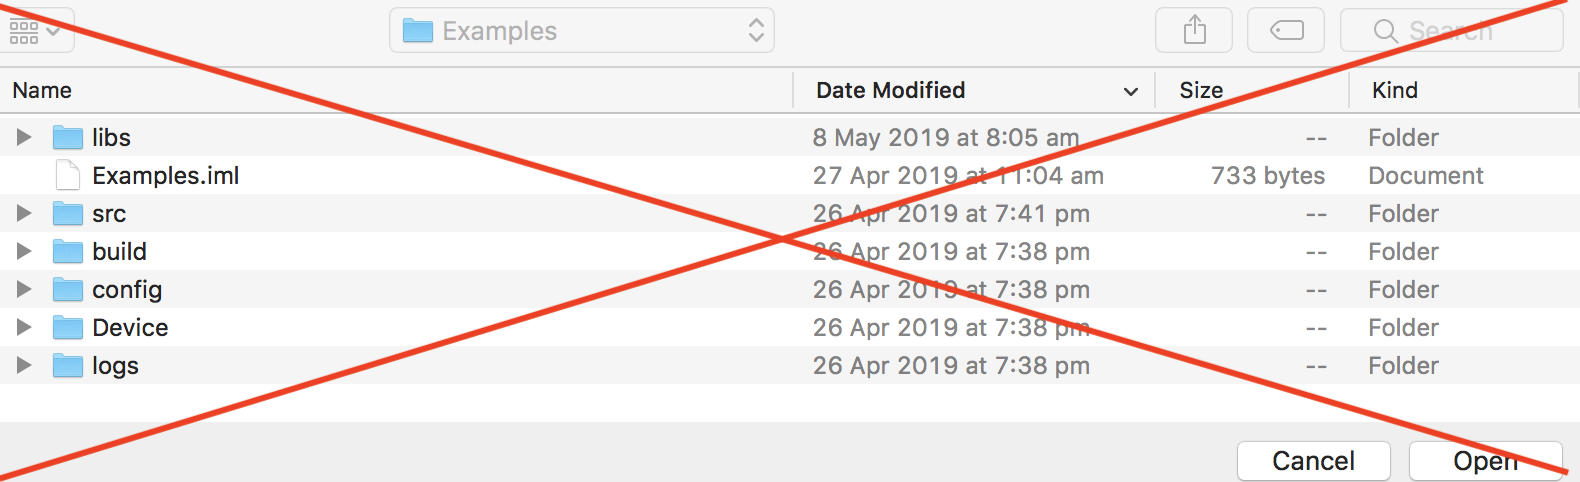
\includegraphics[width=1\columnwidth]{badopen}
	\caption{Incorrect attempt at opening Example Project}
	\label{fig:badopen}
\end{figure}





